\documentclass[11pt, a4paper]{article}
\usepackage[utf8]{inputenc}
\usepackage{fullpage}
\usepackage{graphicx}
\usepackage{markdown}
\usepackage{mathtools}
\usepackage{wrapfig}
\usepackage{tabu}
\usepackage{colortbl}
\usepackage[hidelinks]{hyperref,xcolor}
\usepackage[backend=biber]{biblatex}
\usepackage{adjustbox}
\usepackage{nomencl}
\renewcommand\UrlFont{\color{blue}\rmfamily}
\addbibresource{projectplan.bib}
\addbibresource{prr.bib}
\addbibresource{design.bib}

\title{Preliminary Research Report\\Remote Water Sensing using UAVs}
\author{Robin \textsc{Westerik}}
\newcommand{\supervisors}{Jan \textsc{Bollen}\\Harry \textsc{Futselaar}}

\newcommand{\timePeriod}{February 2022 - June 2022}
\newcommand{\sprint}{Design}
\newcommand{\homepage}{\url{https://github.com/organizations/remotewatersensing/}}
\date{\today}

\makeatletter{}

\makenomenclature
\renewcommand{\nomname}{}

\begin{document}

\begin{titlepage}
  	\newcommand{\HRule}{\rule{\linewidth}{0.3mm}}
	\center
	\textsc{\LARGE Saxion University of Applied Sciences}\\[1.5cm]
	\textsc{\Large International Water Technology}\\[0.5cm]
	\textsc{\large Applied Computer Science Graduation Project}\\[0.5cm]
	\HRule\\[0.4cm]
	{\huge\bfseries \@title}\\[0.4cm]
	\HRule\\[1.5cm]

	%Author(s)
	\begin{minipage}{0.4\textwidth}
		\begin{flushleft}
			\large
			\textit{Author(s)}\\
			\@author % Your name
		\end{flushleft}
	\end{minipage}
	~
	\begin{minipage}{0.4\textwidth}
		\begin{flushright}
			\large
			\textit{Supervisor(s)}\\
			\supervisors
		\end{flushright}
	\end{minipage}
	
% 	If you don't want a supervisor, uncomment the two lines below and comment the code above
% 	{\large\textit{Author(s)}}\\
% 	\@author % Your name

	%Date
	\vfill\vfill
		{\large\today}
    \vfill\vfill
    
    \footnotesize{Time period: \timePeriod}
    \\[0.3cm]
    \footnotesize{Sprint: \sprint}
    \vfill
    \homepage
    
    \vfill
    
    \begin{tabular}{ | l | l | l | l |}
    \hline
    \textbf{Version} & \textbf{Date of change} & \textbf{What is changed?} & \textbf{The reason for the change} \\ \hline
    0.1 & 30-03-2022 & templating & \\
    0.2 & 10-04-2022 & introduction & \\
    0.3 & 11-04-2022 & cad model & \\
    0.4 & 22-04-2022 & sensor selection & \\
    0.5 & 01-05-2022 & MCU + schematic & \\
    0.6 & 17-05-2022 & package design revision 1 & \\
    0.7 & 22-05-2022 & package design revision 2 & \\
    \hline
\end{tabular}
	
	\vfill\vfill
	
\includegraphics[width=0.4\textwidth]{./03_saxionlogo.png}
	\vfill
	 
	\vfill
	
\end{titlepage}

\nomenclature{\(UAV\)}{Unmanned Aerial Vehicle}
\nomenclature{\(BOM\)}{Bill of Materials}
\nomenclature{\(CAD\)}{Computer-Aided Design}
\nomenclature{\(MiB\)}{Mebibyte}
\nomenclature{\(TCP\)}{Transmission Control Protocol}


\tableofcontents
\pagebreak

\section{Abbreviations}
\sffamily\footnotesize
\printnomenclature
\rmfamily\normalsize

\section{Introduction}

In this report, an overview of the working architecture will be designed, along with several prototypes of ways to measure the water quality using drones. This design report will reference a lot of findings from the preliminary research report.

There will be a lot of communication between stakeholder and the project author to discuss the focus of these designs. Sensors will be selected to measure variables referenced in the preliminary research report based on their accuracy and capability to mount on a drone. A suitable drone will be chosen and modelled. Configurations of sensors on the drone will be designed and illustrated.


\newpage
\section{Chosen Drone}
\begin{wrapfigure}{r}{0.3\textwidth}
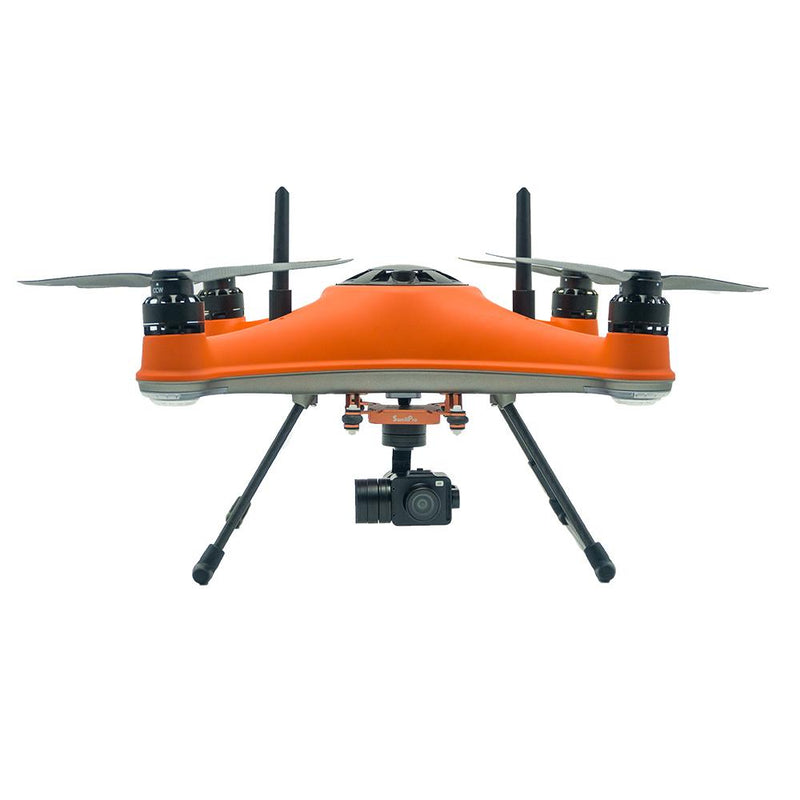
\includegraphics[width=1\linewidth]{21_splashdrone4.png}
\caption{SplashDrone 4}
\end{wrapfigure}
As seen in the Preliminary Research Report, \cite{prr} it turns out that the SwellPro SplashDrone 4 is the best option as a base for the project. While a DIY drone was considered, building a custom drone solution that was also waterproof seemed out of this project's scope.\\

As mentioned, the drone can land in the water, which opens up the possibilities of 2D/3D water quality measurements. The drone has ports on the bottom for connecting hardware via a serial connection. The addons are supplied an output voltage of xV, with a maximum current of yA. \\

This makes it possible to power a microcontroller (using a step down converter), sensors, and even a servo winch. The latter can help when building a sensor enclosure which can move to any depth of water, creating 3D water quality measurements.

\begin{figure}[h]
\centering
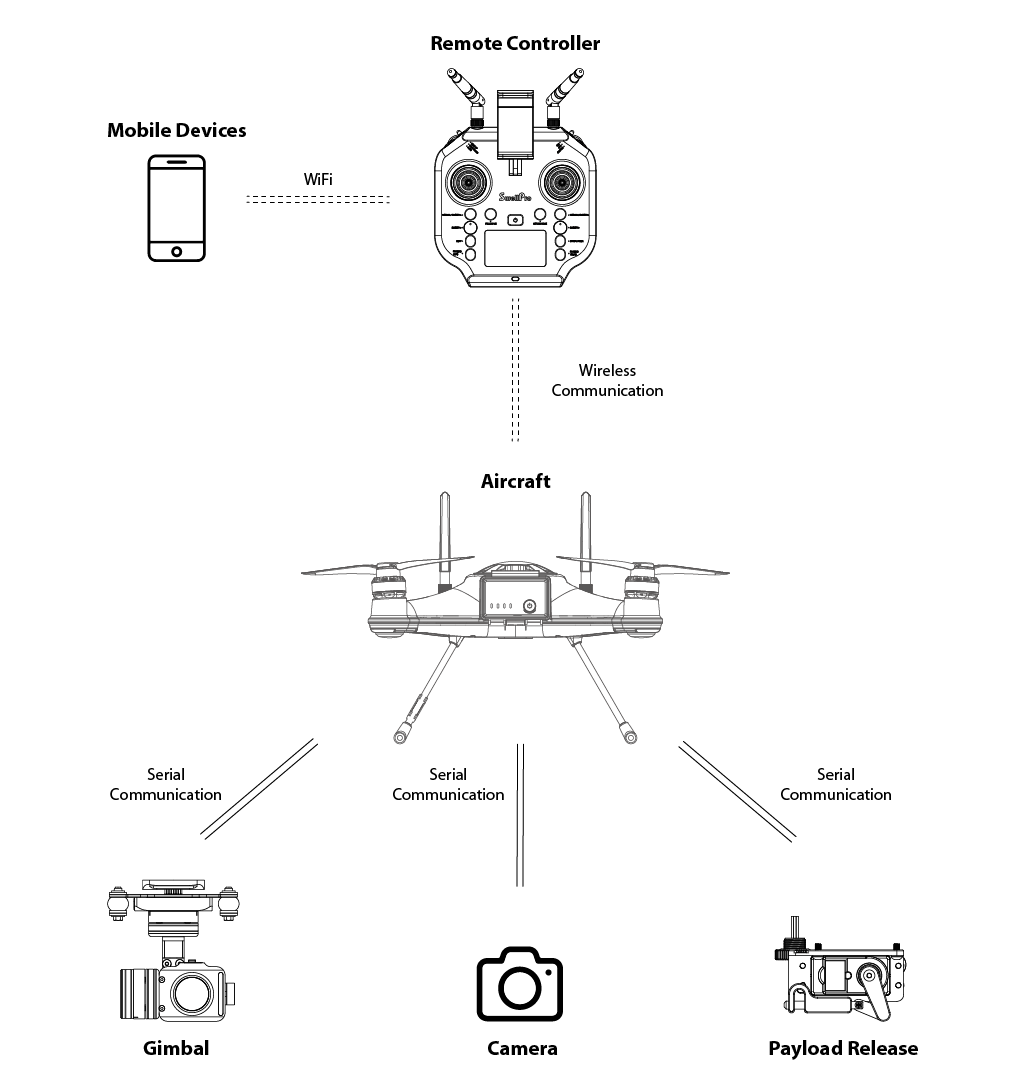
\includegraphics[scale=1.1]{22_controldiagram.png}
\caption{Flight Control Communication Protocol Diagram \cite{swellpronotion}}
\end{figure}

The drone and its addons are entirely controllable via a TCP connection one can have with its remote controller. Data is received and transmitted via Swellpro's "Flight Control Communication Protocol". \cite{swellpronotion}
\newpage
\section{CAD Model}
In order to digitally design add-ons for the SplashDrone 4, the drone has to be modelled using computer-aided design software. To save time, close-range photogrammetry was used to capture the base of the drone.

Photogrammetry can be described as extracting 3D information from photographs. The process involves taking overlapping photographs of an object and converting them into 3D digital models, stitching the images together. 163 high resolution photographs were taken with a DJI Osmo Pocket \cite{osmopocket}, resulting in a raw dataset of 933MiB. The dataset is available on GitHub \cite{dronemodel}. Autodesk ReCap Photo was used for the conversion into a CAD Model \cite{autodeskrecap}

To get the best results, several requirements must be met. Creative ways were found to pass these requirements when capturing the drone at home:

\begin{center}
\begin{tabular}{ |c|c| } 
 \hline
 Requirement & Fix  \\ 
 \hline
 Object must have texture & Smear removable shoe polish on the body \\ 
 Object must not be reflective & Mask the reflective dome with toilet paper \\ 
 Base must have variation & Use colourful bed sheets \\ 
 Lighting conditions must be consistent & Use a beach umbrella to diffuse the sun light \\ 
 \hline
\end{tabular}
\end{center}

Initial conversion seemed to be good, though some small patching had to be done, especially on the motors:

\begin{figure}[h]
  \centering
  \begin{minipage}[b]{0.4\textwidth}
    \includegraphics[width=\textwidth]{31_dphoto.jpg}
    \caption{Original photo \cite{dronemodel}}
  \end{minipage}
  \hfill
  \begin{minipage}[b]{0.5\textwidth}
    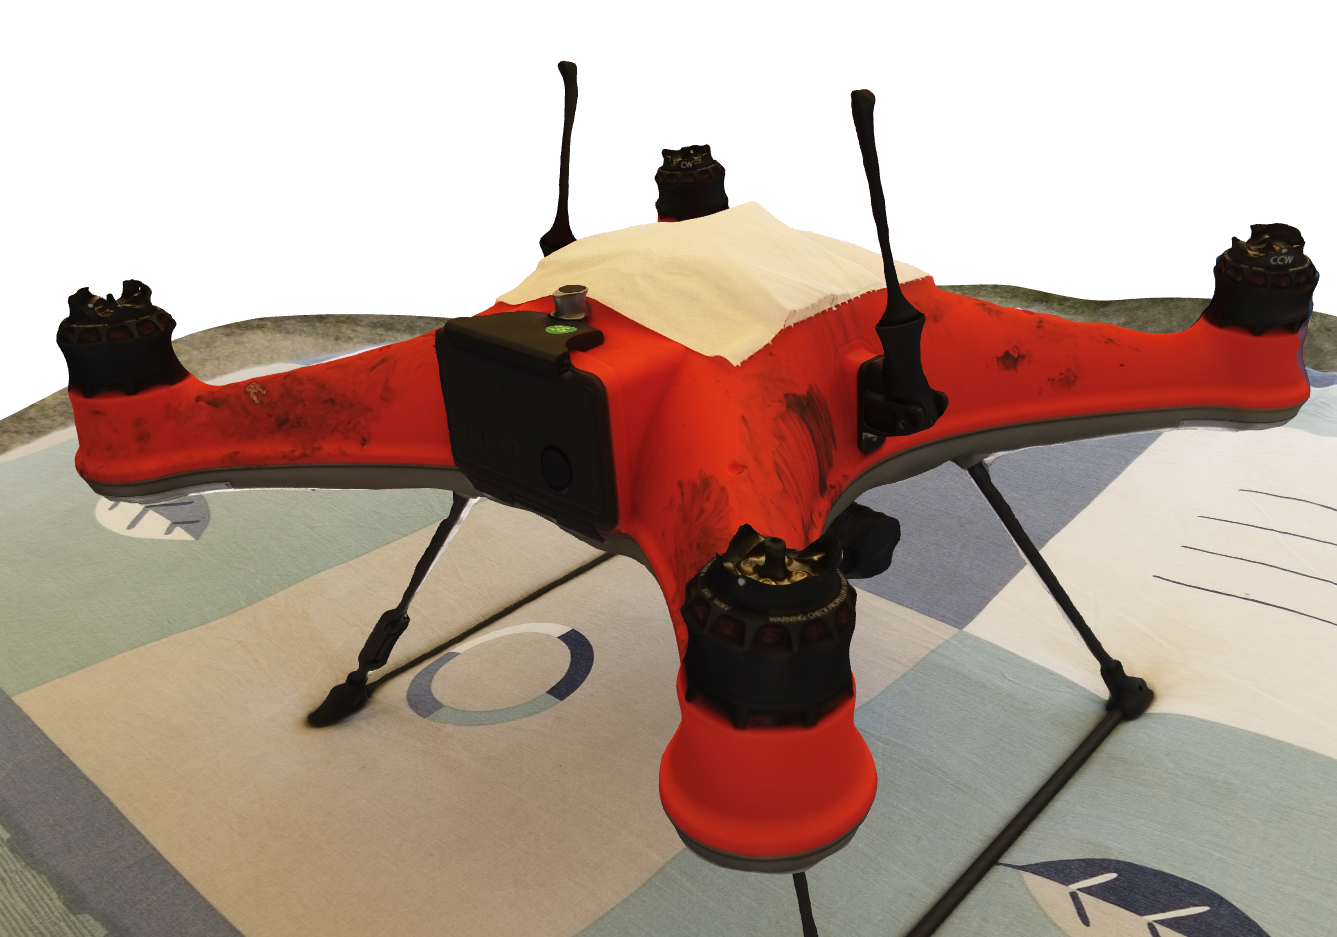
\includegraphics[width=\textwidth]{32_dmodel.png}
    \caption{3D Model \cite{dronemodel}}
  \end{minipage}
\end{figure}

The program failed to capture the gimbal of the drone accurately as it was able to move freely during capture. The bottom has been roughly reworked later on in CAD software, leading to the following result:

\begin{figure}[h]
\centering
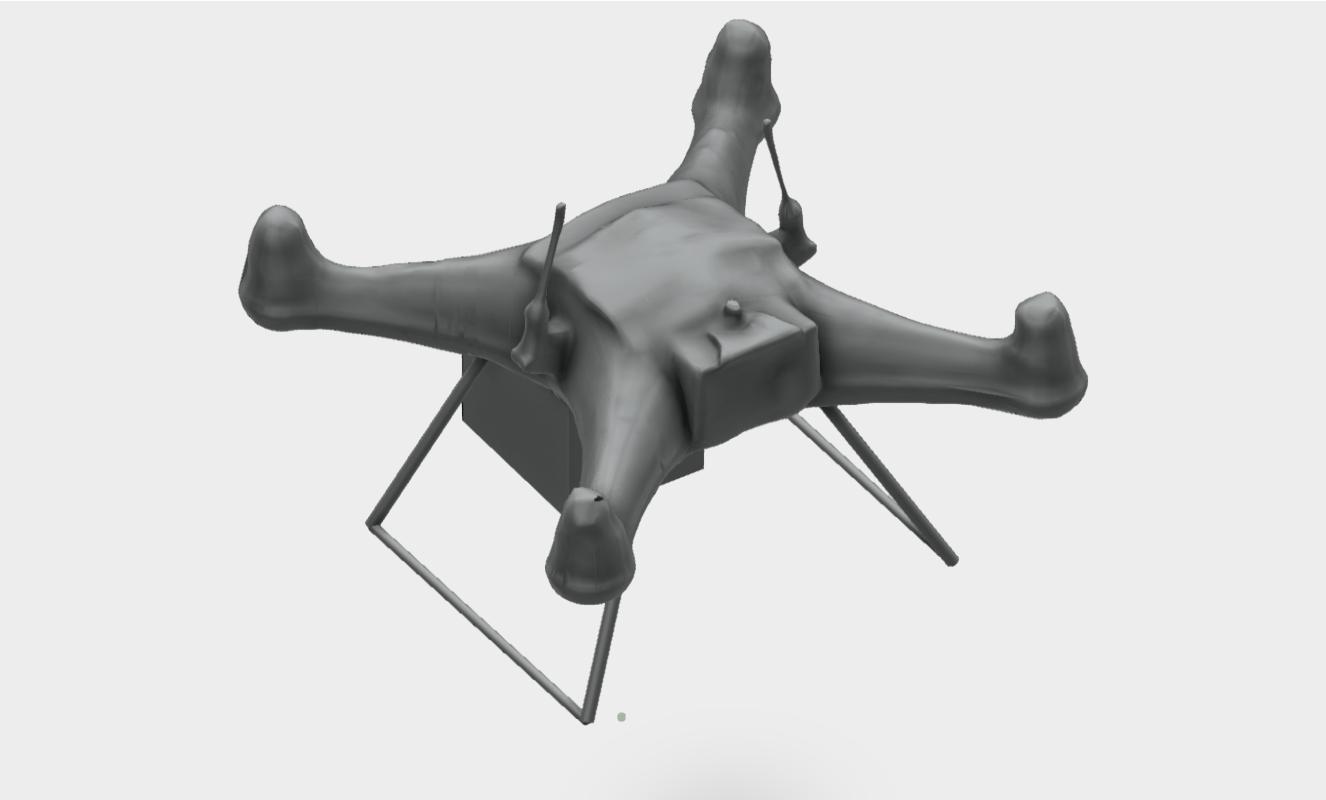
\includegraphics[scale=0.1]{33_dcadmodel.png}
\caption{Final CAD Model \cite{dronemodel}}
\end{figure}

As the gimbal of the drone is not of any importance, it is not modelled and instead modelled as a 3D box. While the model is not perfect, it is adequate for our use case.


\newpage
\section{Sensors}
After careful consideration, 4 water quality parameters are chosen to be monitored: turbidity, acidity, conductivity, and temperature. This set of sensors will help monitoring both the salinization issues and acidity issues at hand

\subsection{Turbidity}
To measure the turbidity, the DFRobot SEN0189 \cite{SEN0189} was chosen because of it's availability and ease of hooking up.
\begin{table}[h!]
	\centering
	\adjustimage{height=4cm,valign=c}{41_sen0189.jpg}\quad
	\begin{tabular}{| l | l |}
    \hline
    Protocol & Analog\\
    Operating Temperature & 5-90 ℃ \\
    Operating Range &  0-3000NTU\\
    Response time & Within 500ms \\
    Supply Voltage & 0V-4.5V \\
    Software library included & yes \\
    Availability & 3-5 Days \\
    \hline
	\end{tabular}
\end{table}

\subsection{Acidity}
To measure the acidity, the DFRobot SEN0169 V2 Pro \cite{SEN0169V2} was chosen because of it's ease of hooking up and existing software libraries.
\begin{table}[h!]
	\centering
	\adjustimage{height=4cm,valign=c}{42_gravityv2pro.jpg}\quad
	\begin{tabular}{| l | l |}
    \hline
    Interface & Analog \\
    Measurement Range & 0-14 pH \\
    Measurement Accuracy &  0.1pH \\
    Response time & Within 1min \\
    Supply Voltage & 3.3V-5V \\
    Software library included & yes \\
    Long term immersion & yes \\
    Availability & 3-5 Working Days \\
    \hline
	\end{tabular}
\end{table}

\subsection{Conductivity}
To measure the conductivity, the DFRobot DFR0300H \cite{DFR0300H} was chosen because of its availability and included software library.
\begin{table}[h!]
	\centering
	\adjustimage{height=4cm,valign=c}{43_dfr0300h.jpg}\quad
	\begin{tabular}{| l | l |}
    \hline
    Protocol & Analog\\
    Measurement Accuracy &  5\% FSR\\
    Supply Voltage & 3.3-5V\\
    Support Detection Range & 10~100ms/cm\\
    Software library included & yes \\
    Probe included & yes \\
    Availability & 3-5 Working days \\
    \hline
	\end{tabular}
\end{table}

\newpage
\subsection{Temperature}
To measure the temperature, the DFRobot DFR0198/DS18B20 \cite{DFR0198} was chosen because of the accuracy and fast response times.
\begin{table}[h!]
	\centering
	\adjustimage{height=4cm,valign=c}{44_dfr0198.jpg}\quad
	\begin{tabular}{| l | l |}
    \hline
    Protocol & 1-Wire\\
    Measurement Range & -10-85 ℃ \\
    Measurement Accuracy &  0.5 ℃ \\
    Response time & Within 750ms \\
    Supply Voltage & 3.3V-5V \\
    Software library included & yes \\
    Availability & 3-5 Working Days \\
    \hline
	\end{tabular}
\end{table}

\subsection{MCU}
An Arduino Uno derivative is used as the MCU to communicate the sensors and the drone. The board  (Vietduino \cite{vietduino}) is based on the ATmega328P microcontroller, and has a CP2102 UART-to-Serial interface. The Vietduino has superior power delivery over the original Arduino Uno. While a more performant microcontroller could have been used, the Vietduino was chosen because of the popular form factor and the ease of rapid prototyping. The popularity of the board makes for an excellent base for people working on this project in the future.

\begin{figure}[h]
  \centering
  \begin{minipage}[b]{0.4\textwidth}
    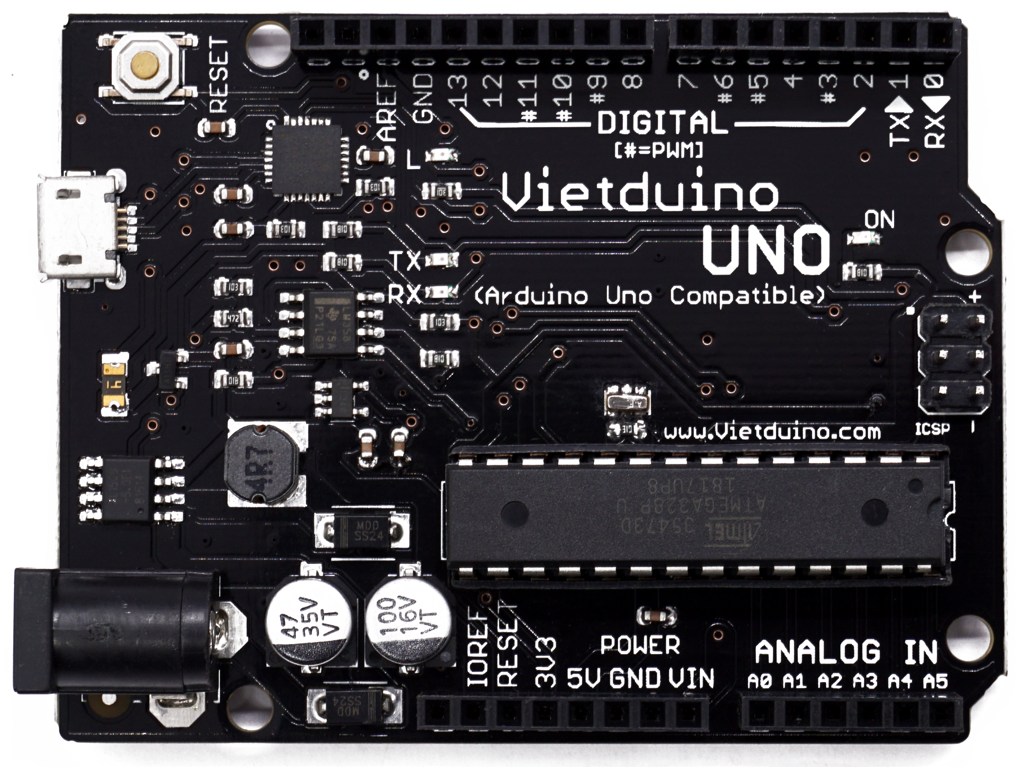
\includegraphics[width=\textwidth]{45_vietduino.png}
    \caption{Vietduino \cite{vietduino}}
  \end{minipage}
  \hfill
  \begin{minipage}[b]{0.5\textwidth}
    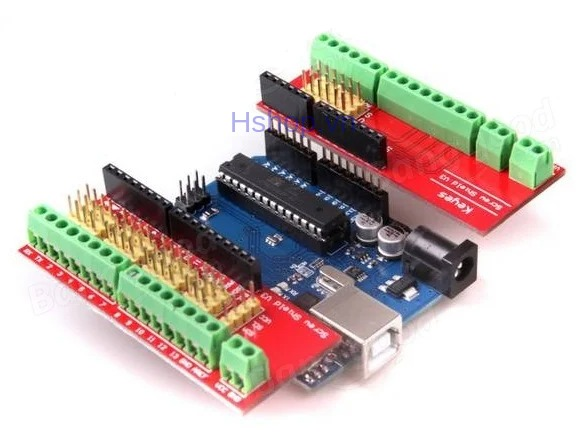
\includegraphics[width=\textwidth]{46_screwshield.jpeg}
    \caption{Screw Shield V3 \cite{screwshield}}
  \end{minipage}
\end{figure}

A screw shield was used to help with cable management and rapid prototyping. This screw shield exposes the digital and analog pins on the Arduino alongside the ground and voltage rail. This way, there is no need for any breadboard.

\newpage
\subsection{Schematics}
In the illustration below one can find the schematics of the sensors and the microcontroller board.
\begin{figure}[h]
\centering
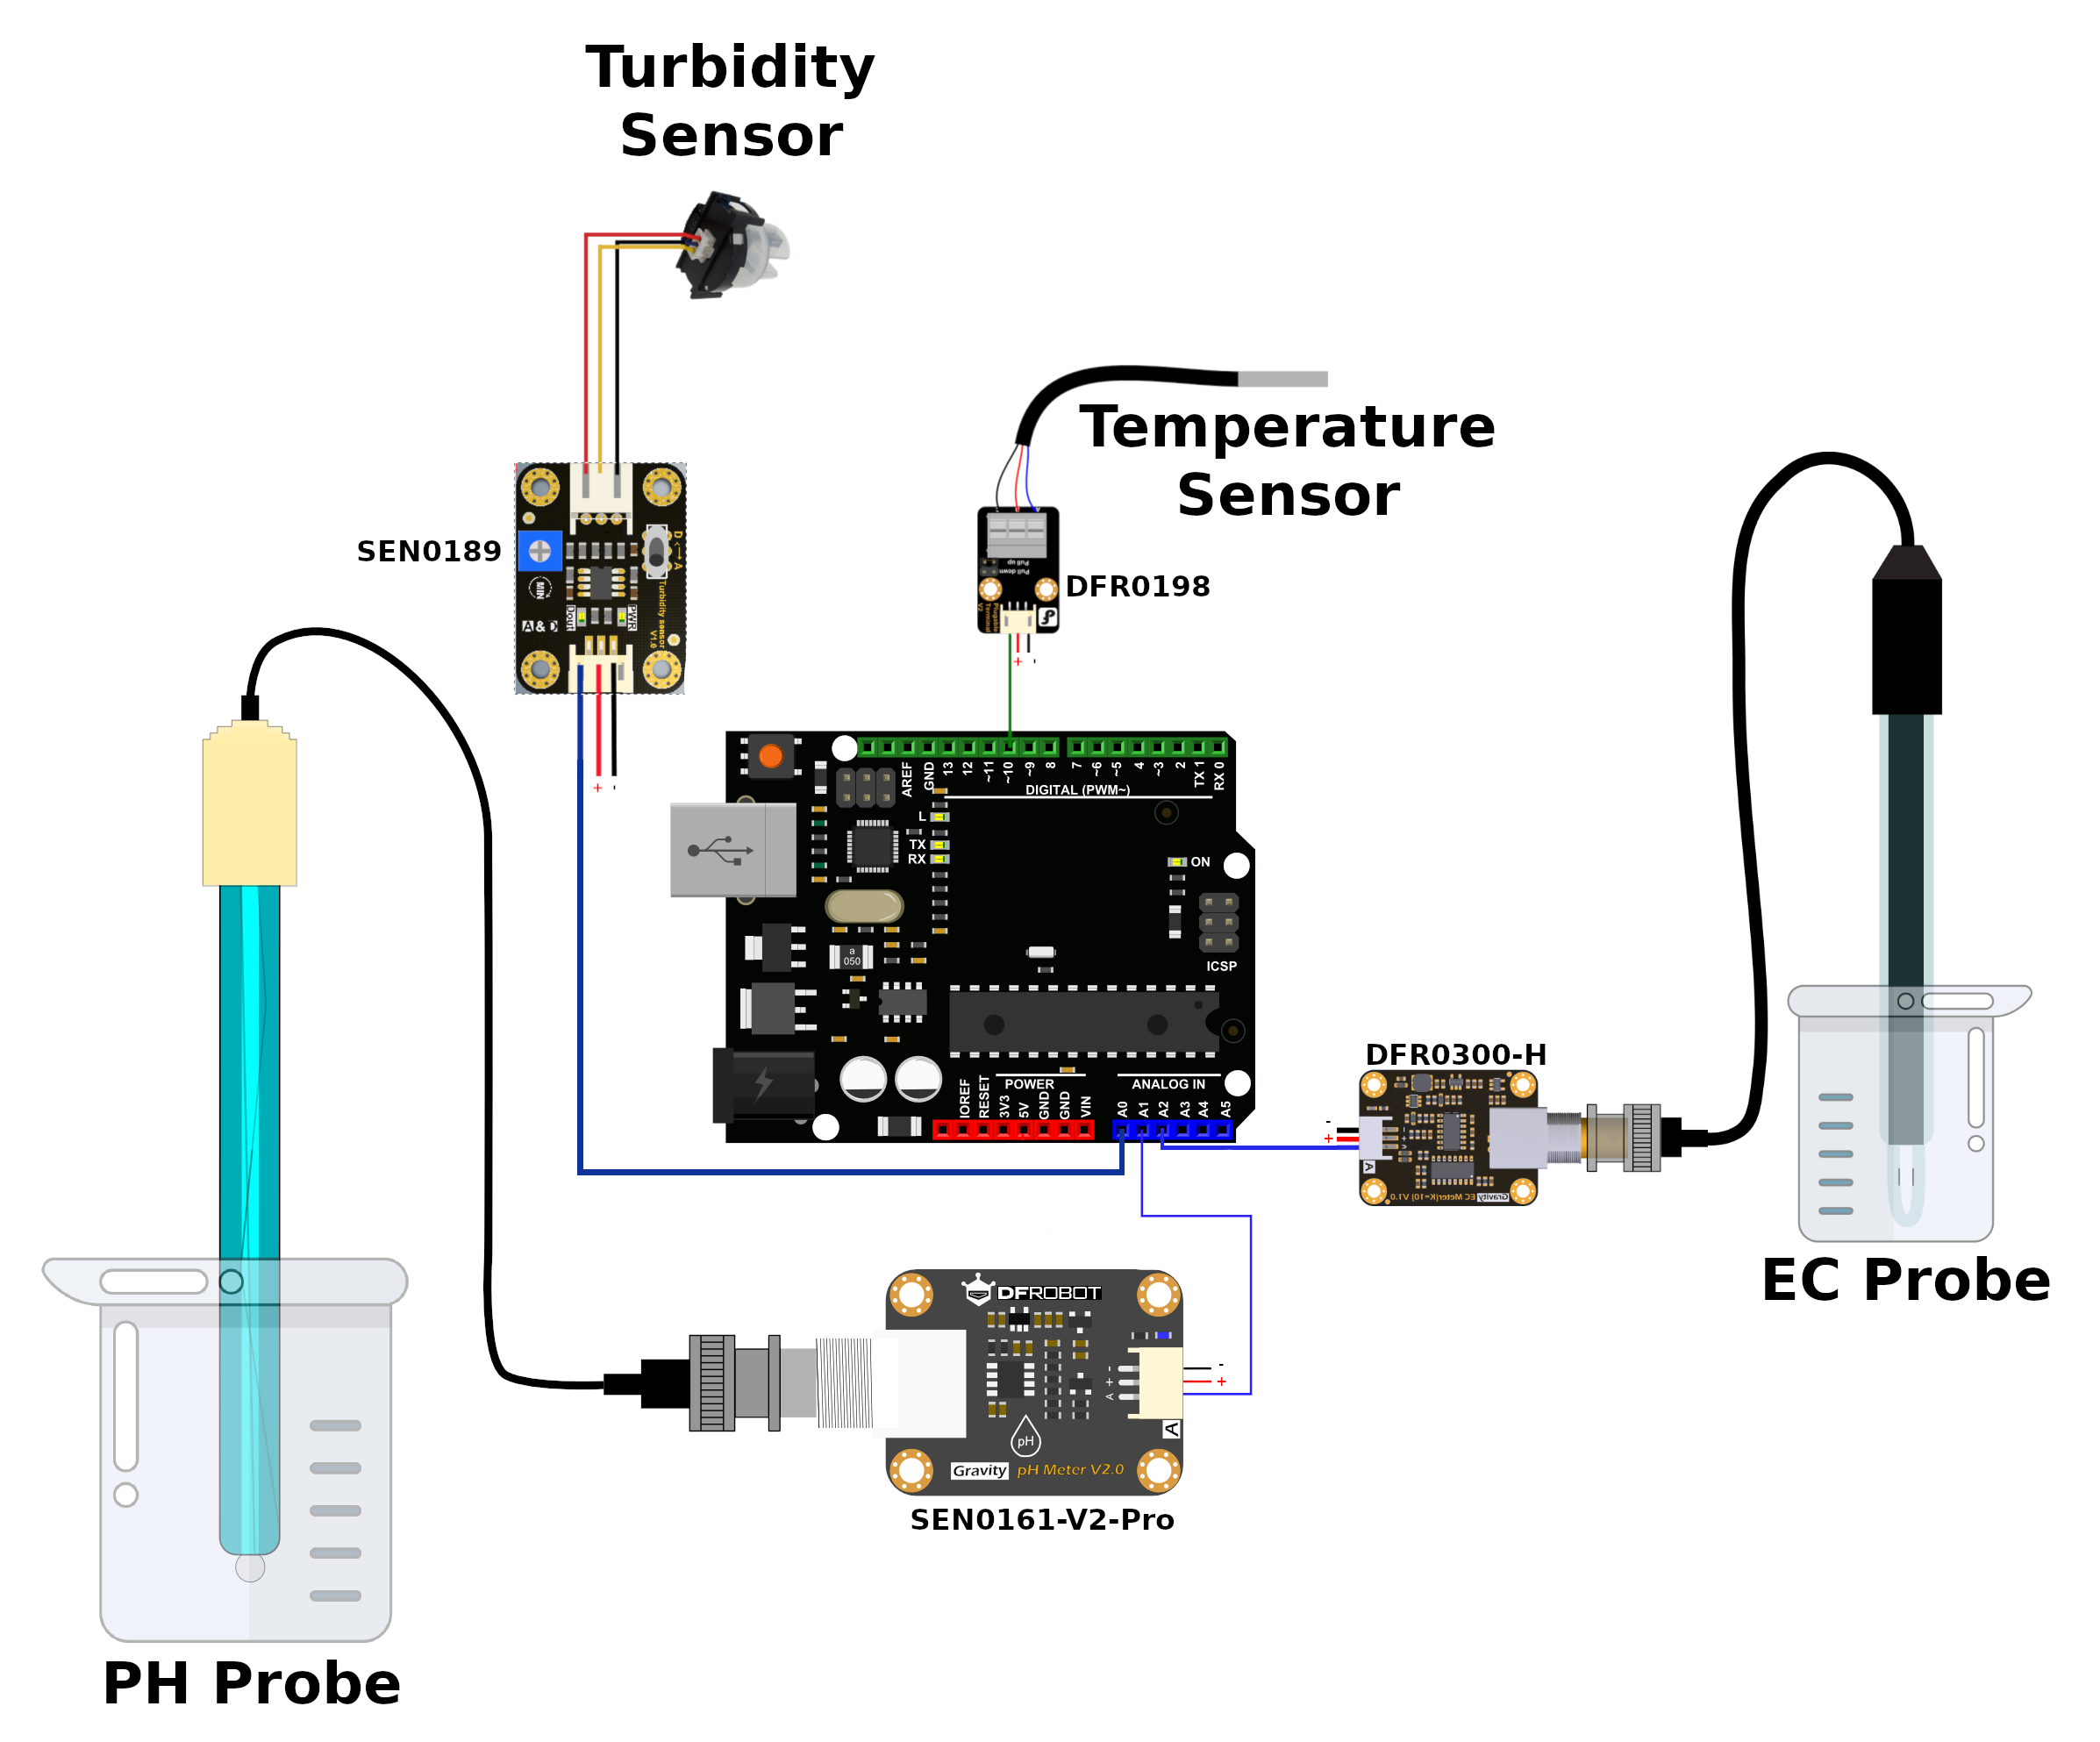
\includegraphics[scale=0.8]{47_schematic.png}
\caption{MCU and sensors schematic}
\end{figure}


\newpage
\section{Sensor Package Design}
The sensors, the micro controller unit and the additional electronics are all combined in the sensor package. Throughout testing there has been revisions on this sensor package.\\

In the Preliminary Research Report it was stated that the project would make use out of 3D designs. As it turns out that the sensor package didn't require any unique shapes, it made better sense to edit existing enclosures, like project boxes.

\subsection{Revision 1}
The initial idea was to the components in one plastic enclosure. A project box was acquired at the Nhat Tao market and holes were drilled out at the side of the box to make mounts for the the turbidity, acidity, and conductivity sensors.

\begin{figure}[h]
\centering
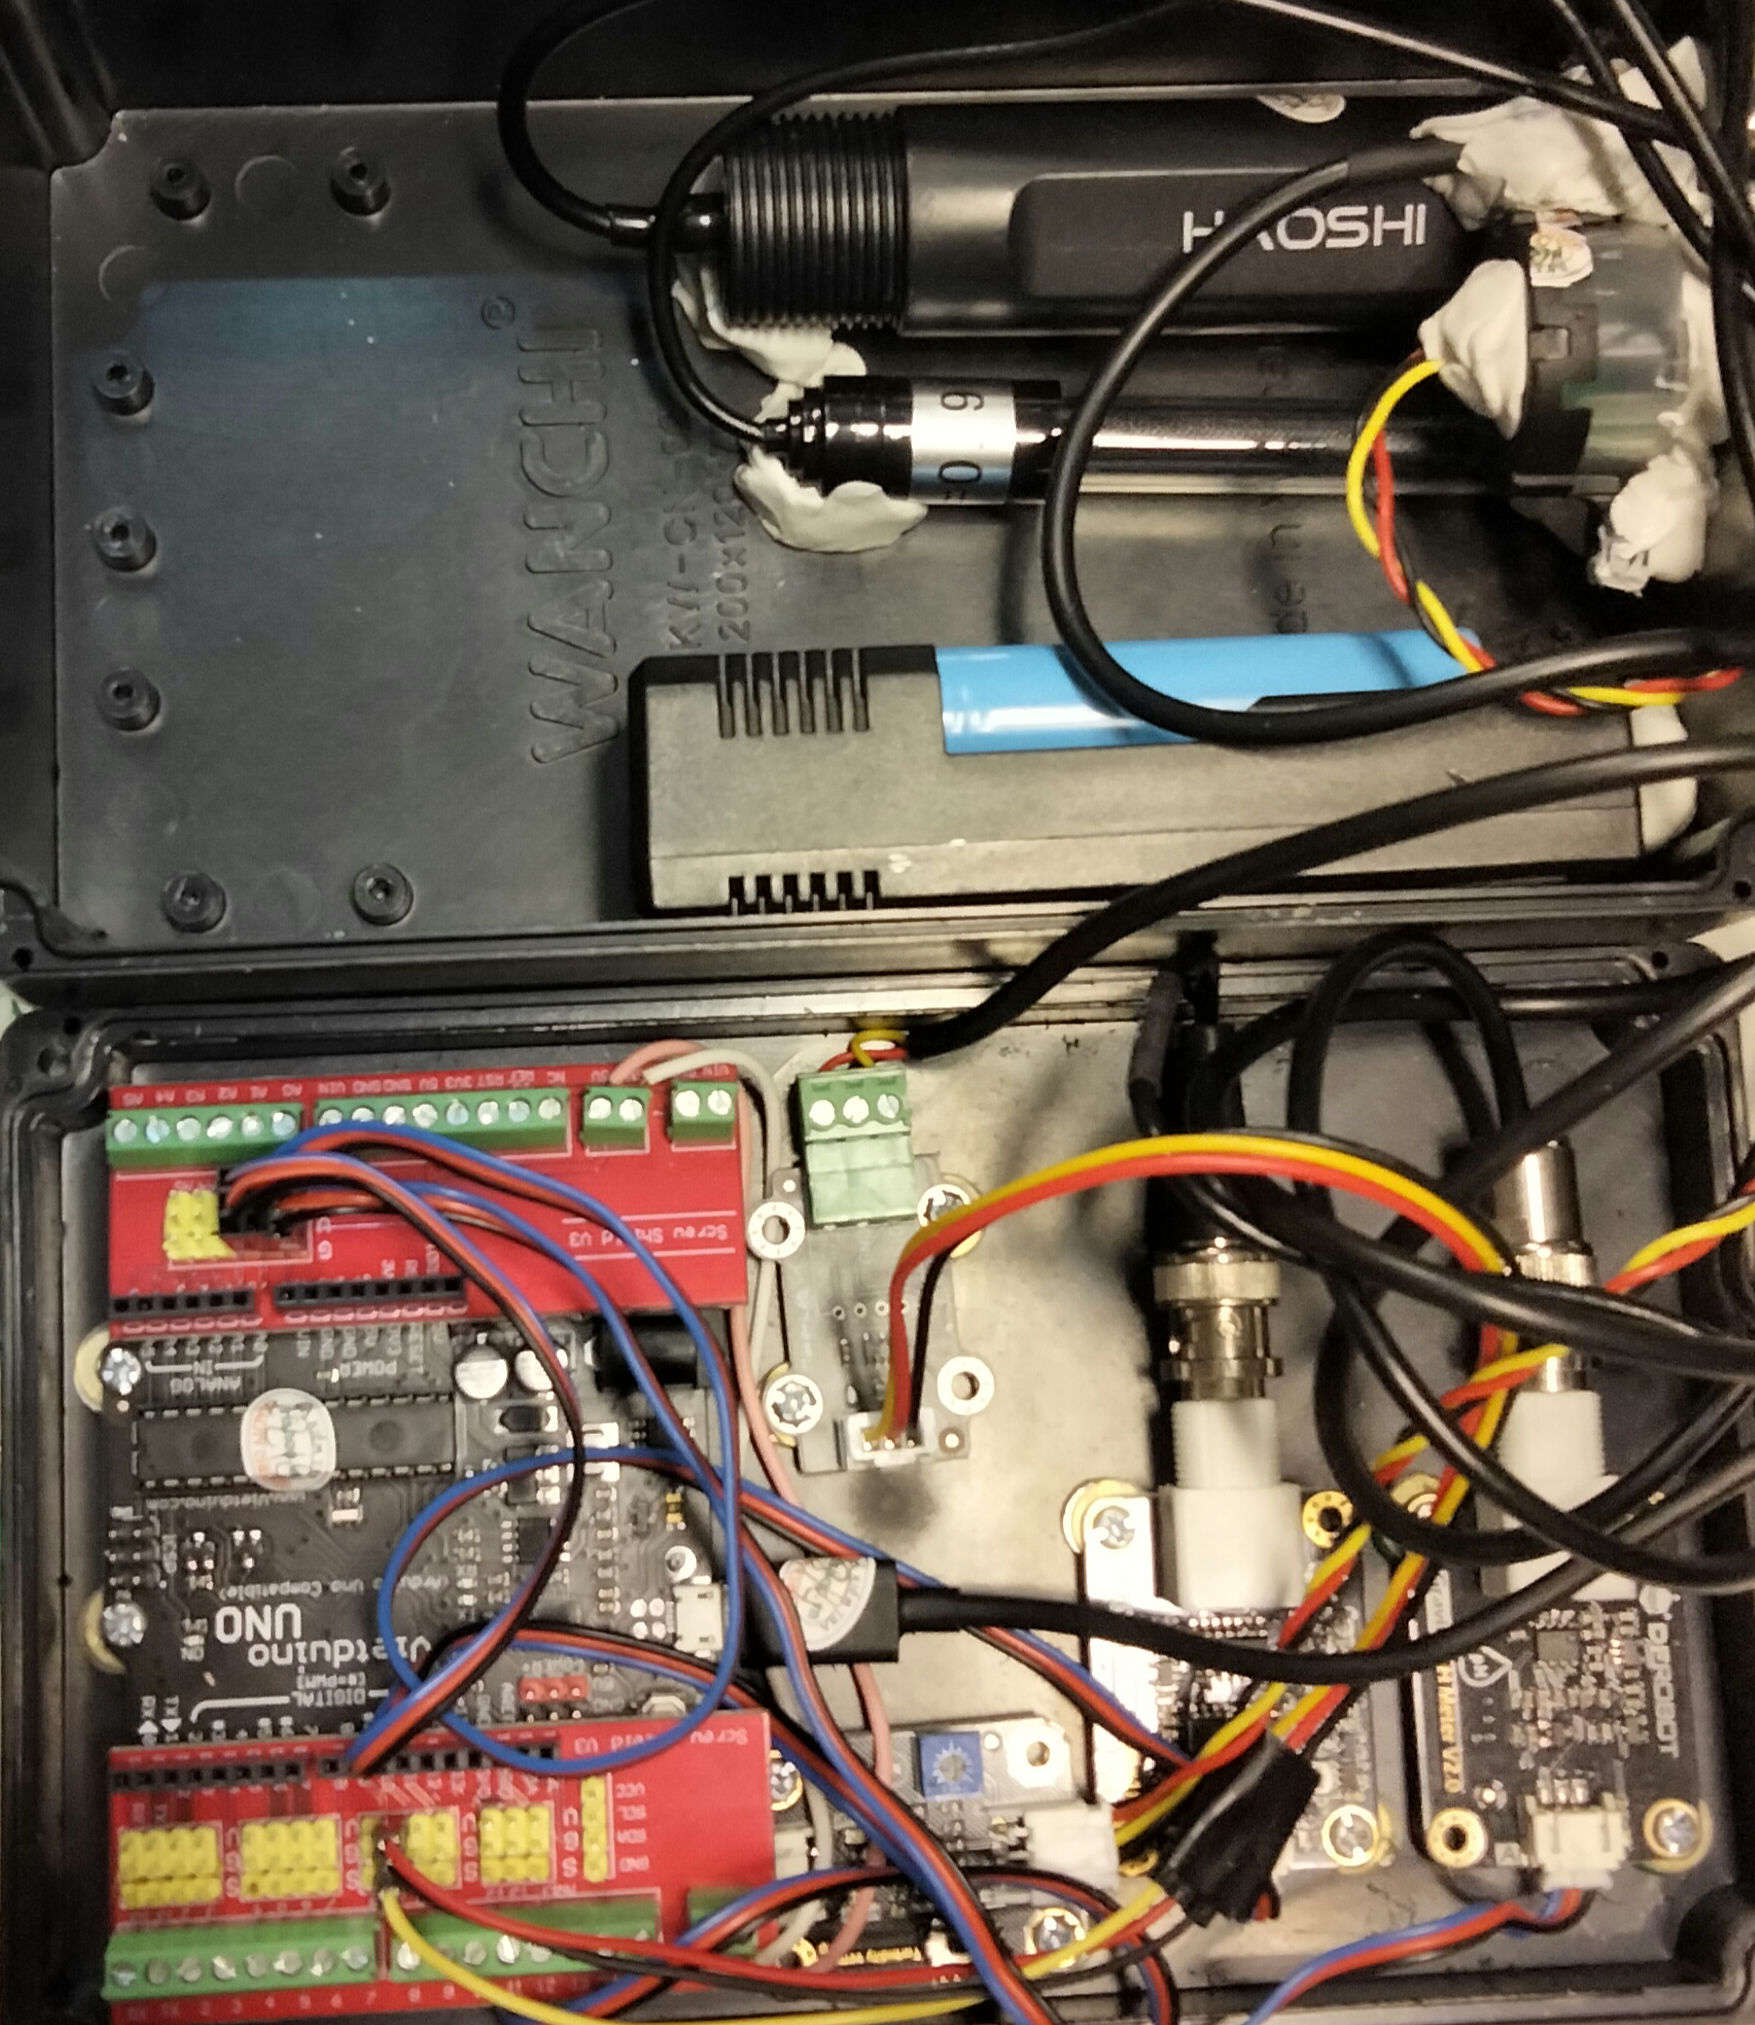
\includegraphics[scale=0.1]{51_rev1.jpg}
\caption{Inside of the first revision}
\end{figure}

The bottom of the box has screw holes drilled out for mounting the pcbs in the case. To prevent water from coming into the enclosure, O-rings are used along with sticky tack. Rubber inserts were used to close down the box. After some preliminary testing, it turned out that some water still leaked into the enclosure while fully submerged.
\newpage
\subsection{Revision 2}
On the second revision, a different approach was taken. The sensitive non-waterproof PCBs were covered by a two-part epoxy, so that even if water would come into the enclosure, it would not be likely to short any circuits.\\

The PCBs are mounted on a metal holed sheet covered with conductive tape. This way, the entire box could be replaced easily in the future without dismounting any PCB's. A swivel is used to lead the cables waterproof outside the enclosure.

\begin{figure}[h]
\centering
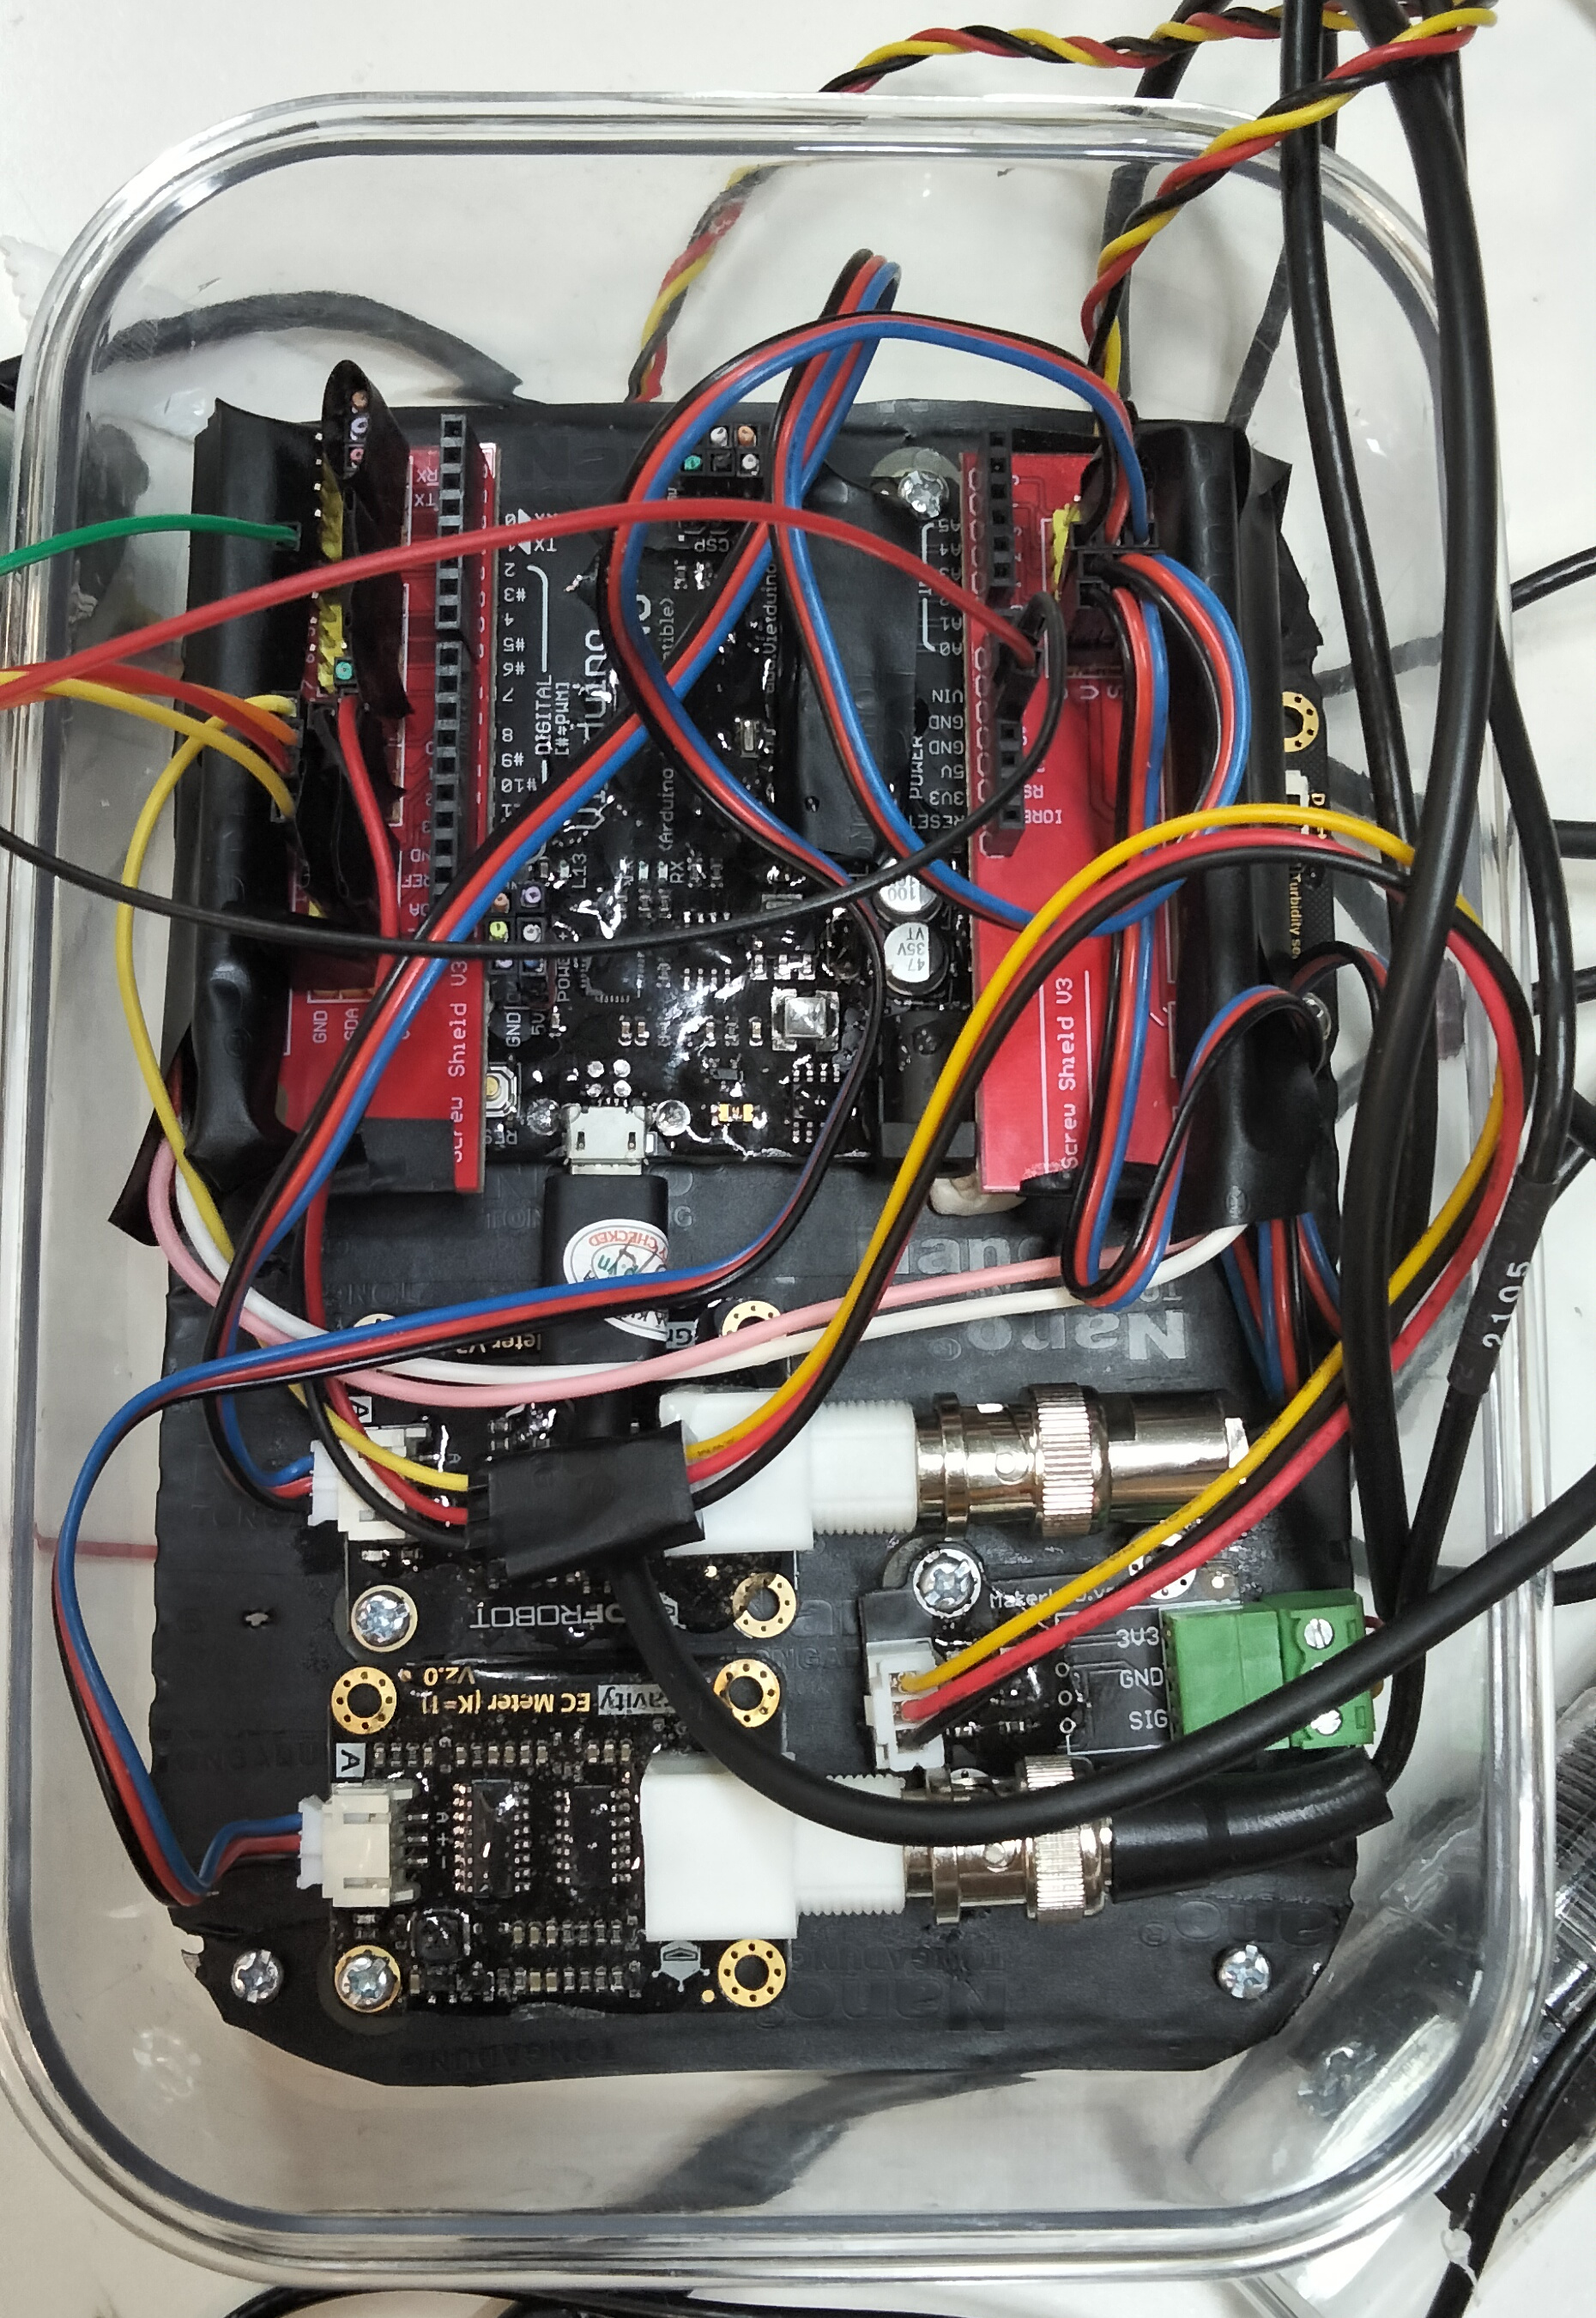
\includegraphics[scale=0.4]{52_rev2.jpg}
\caption{Inside of the second revision}
\end{figure}

The sensor probes are placed outside the enclosure on a rack underneath the drone to be fully submerged in the water, while the enclosure is placed on the drone above the water.

\newpage
\subsection{Secchi Disk}
To determine the turbidity, a secchi disk is used. This disk was made from an used 30cm record. Tape was used to make the black and white sides. An eye bolt was used to make a hole for the rope to attach. The secchi disk is attached to the middle of the bottom grid of the drone.

\begin{figure}[h]
\centering
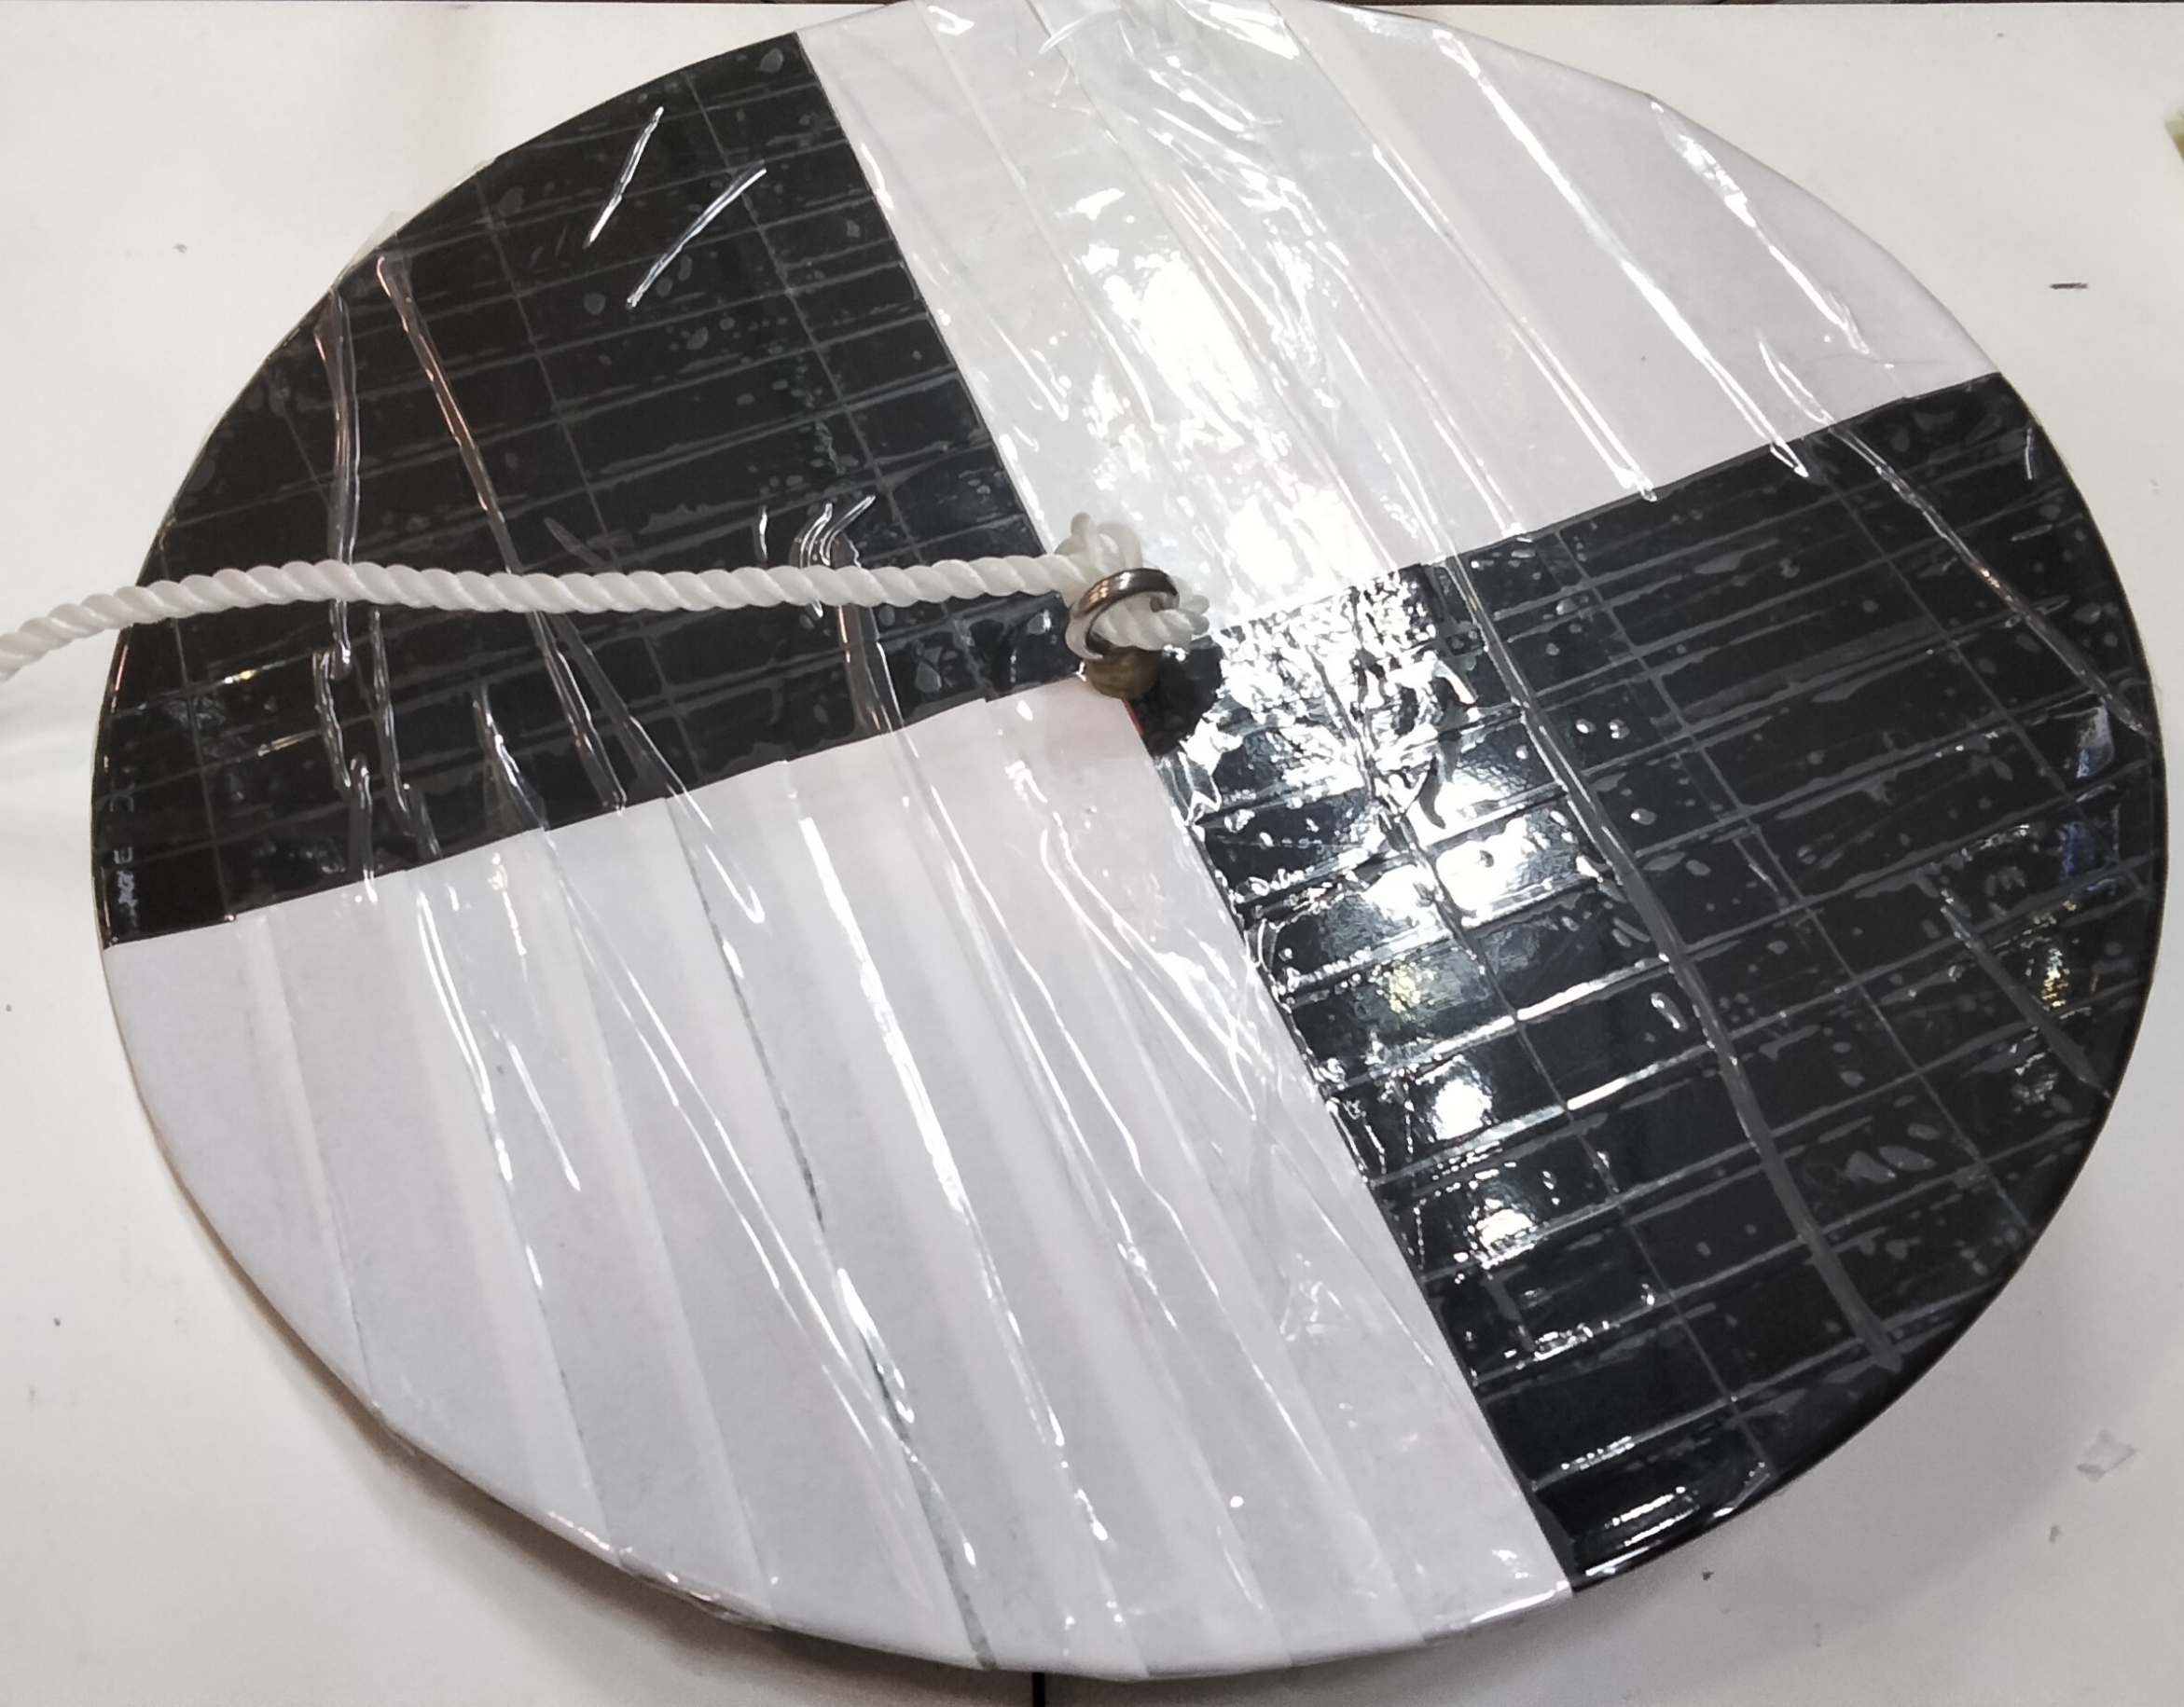
\includegraphics[scale=0.1]{53_secchi.jpg}
\caption{DIY Secchi Disk}
\end{figure}

\newpage
\printbibliography 

\end{document}